% =============================================================================
% The Rhetoric of Decks
% A Beamer Presentation on Sequential Visual Persuasion
% =============================================================================

\documentclass[aspectratio=169,11pt]{beamer}

% -----------------------------------------------------------------------------
% PACKAGES
% -----------------------------------------------------------------------------
\usepackage[utf8]{inputenc}
\usepackage[T1]{fontenc}
\usepackage{lmodern}
\usepackage{microtype}
\usepackage{amsmath,amssymb}
\usepackage{booktabs}
\usepackage{graphicx}
\usepackage{tikz}
\usepackage{pgfplots}
\usepackage{xcolor}
\usepackage{fontawesome5}
\usepackage{ragged2e}
\usepackage{setspace}
\usepackage{colortbl}
\usepackage{array}
\usepackage{multirow}
\usepackage{hyperref}

\usetikzlibrary{shapes.geometric, arrows.meta, positioning, calc, backgrounds,
                decorations.pathreplacing, shadows, fadings}
\pgfplotsset{compat=1.18}

% -----------------------------------------------------------------------------
% COLOR PALETTE - Professional, warm, sophisticated
% -----------------------------------------------------------------------------
\definecolor{DeepNavy}{HTML}{2E4057}
\definecolor{Teal}{HTML}{048A81}
\definecolor{WarmOrange}{HTML}{E85D04}
\definecolor{SoftPurple}{HTML}{9D4EDD}
\definecolor{WarmGray}{HTML}{6C757D}
\definecolor{LightGray}{HTML}{E9ECEF}
\definecolor{Cream}{HTML}{FBF8F1}
\definecolor{DeepRed}{HTML}{D62828}
\definecolor{Gold}{HTML}{D4A03A}
\definecolor{SoftWhite}{HTML}{FAFAFA}

% Set beamer colors
\setbeamercolor{normal text}{fg=DeepNavy,bg=SoftWhite}
\setbeamercolor{structure}{fg=DeepNavy}
\setbeamercolor{alerted text}{fg=WarmOrange}
\setbeamercolor{example text}{fg=Teal}

\setbeamercolor{palette primary}{bg=DeepNavy,fg=white}
\setbeamercolor{palette secondary}{bg=Teal,fg=white}
\setbeamercolor{palette tertiary}{bg=WarmOrange,fg=white}

\setbeamercolor{frametitle}{fg=DeepNavy,bg=SoftWhite}
\setbeamercolor{title}{fg=DeepNavy}
\setbeamercolor{subtitle}{fg=WarmGray}
\setbeamercolor{author}{fg=WarmGray}
\setbeamercolor{date}{fg=WarmGray}

\setbeamercolor{block title}{bg=DeepNavy,fg=white}
\setbeamercolor{block body}{bg=LightGray,fg=DeepNavy}
\setbeamercolor{block title alerted}{bg=WarmOrange,fg=white}
\setbeamercolor{block body alerted}{bg=LightGray,fg=DeepNavy}
\setbeamercolor{block title example}{bg=Teal,fg=white}
\setbeamercolor{block body example}{bg=LightGray,fg=DeepNavy}

% Item colors
\setbeamercolor{itemize item}{fg=Teal}
\setbeamercolor{itemize subitem}{fg=WarmOrange}
\setbeamercolor{enumerate item}{fg=Teal}

% -----------------------------------------------------------------------------
% FONTS AND TYPOGRAPHY
% -----------------------------------------------------------------------------
\usefonttheme{professionalfonts}
\setbeamerfont{title}{size=\LARGE,series=\bfseries}
\setbeamerfont{subtitle}{size=\normalsize,series=\mdseries}
\setbeamerfont{frametitle}{size=\Large,series=\bfseries}
\setbeamerfont{framesubtitle}{size=\small,series=\mdseries}
\setbeamerfont{author}{size=\normalsize}
\setbeamerfont{date}{size=\small}
\setbeamerfont{footnote}{size=\tiny}

% -----------------------------------------------------------------------------
% BEAMER TEMPLATE CUSTOMIZATION
% -----------------------------------------------------------------------------
\setbeamertemplate{navigation symbols}{}
\setbeamertemplate{headline}{}

% Custom frame title
\setbeamertemplate{frametitle}{%
    \vspace{0.5cm}
    \begin{beamercolorbox}[wd=\paperwidth,leftskip=0.8cm]{frametitle}
        \usebeamerfont{frametitle}\insertframetitle
        \ifx\insertframesubtitle\empty\else
            \\[0.1cm]
            {\usebeamerfont{framesubtitle}\usebeamercolor[fg]{subtitle}\insertframesubtitle}
        \fi
    \end{beamercolorbox}
}

% Minimal footline with just page number
\setbeamertemplate{footline}{%
    \hfill
    \begin{beamercolorbox}[wd=3cm,ht=2.5ex,dp=1ex,right,rightskip=0.5cm]{page number}
        \usebeamercolor[fg]{WarmGray}\scriptsize\insertframenumber
    \end{beamercolorbox}
    \vspace{0.3cm}
}

% Itemize bullets
\setbeamertemplate{itemize item}{\footnotesize\raisebox{0.3ex}{\tikz\fill[Teal] (0,0) circle (0.5ex);}}
\setbeamertemplate{itemize subitem}{\footnotesize\raisebox{0.3ex}{\tikz\fill[WarmOrange] (0,0) circle (0.4ex);}}

% Enumerate
\setbeamertemplate{enumerate item}{\textcolor{Teal}{\insertenumlabel.}}

% Remove margins from block
\addtobeamertemplate{block begin}{}{\vspace*{-0.5\baselineskip}}
\addtobeamertemplate{block end}{}{\vspace*{-0.5\baselineskip}}

% -----------------------------------------------------------------------------
% CUSTOM COMMANDS
% -----------------------------------------------------------------------------
\newcommand{\emphcolor}[1]{\textcolor{WarmOrange}{\textbf{#1}}}
\newcommand{\tealtext}[1]{\textcolor{Teal}{#1}}
\newcommand{\graytext}[1]{\textcolor{WarmGray}{#1}}
\newcommand{\bigidea}[1]{%
    \begin{center}
    \Large\color{DeepNavy}\textbf{#1}
    \end{center}
}

% Transition slides
\newcommand{\transitionslide}[2]{%
    \begin{frame}[plain]
        \begin{tikzpicture}[remember picture,overlay]
            \fill[DeepNavy] (current page.south west) rectangle (current page.north east);
            \node[anchor=center,text=white,font=\Huge\bfseries,text width=0.8\paperwidth,align=center]
                at (current page.center) {#1};
            \node[anchor=center,text=LightGray,font=\large,text width=0.8\paperwidth,align=center,
                  below=1cm of current page.center] {#2};
        \end{tikzpicture}
    \end{frame}
}

% Quote environment
\newenvironment{quoteslide}[1]{%
    \begin{frame}[plain]
    \begin{tikzpicture}[remember picture,overlay]
        \fill[Cream] (current page.south west) rectangle (current page.north east);
        \node[anchor=west,text=Teal,font=\fontsize{60}{60}\selectfont,opacity=0.2]
            at ([xshift=1cm,yshift=-1cm]current page.north west) {``};
        \node[anchor=east,text=Teal,font=\fontsize{60}{60}\selectfont,opacity=0.2]
            at ([xshift=-1cm,yshift=1cm]current page.south east) {''};
    \end{tikzpicture}
    \vspace{1.5cm}
    \begin{center}
    \begin{minipage}{0.75\textwidth}
    \centering
    \Large\color{DeepNavy}\itshape
}{%
    \end{minipage}
    \end{center}
    \end{frame}
}

% -----------------------------------------------------------------------------
% DOCUMENT METADATA
% -----------------------------------------------------------------------------
\title{The Rhetoric of Decks}
\subtitle{Sequential Visual Persuasion in the Age of AI}
\author{A Theory of Effective Presentation}
\date{}

% =============================================================================
% DOCUMENT BEGINS
% =============================================================================
\begin{document}

% -----------------------------------------------------------------------------
% TITLE SLIDE
% -----------------------------------------------------------------------------
{
\setbeamertemplate{footline}{}
\begin{frame}[plain]
\begin{tikzpicture}[remember picture,overlay]
    % Background gradient effect using rectangles
    \fill[DeepNavy] (current page.south west) rectangle (current page.north east);

    % Decorative geometric elements
    \fill[Teal,opacity=0.3] ([xshift=-2cm,yshift=-3cm]current page.north east) circle (5cm);
    \fill[WarmOrange,opacity=0.2] ([xshift=3cm,yshift=2cm]current page.south west) circle (4cm);

    % Subtle grid pattern
    \foreach \i in {-5,-4,...,15} {
        \draw[white,opacity=0.03,line width=0.5pt]
            ([xshift=\i cm]current page.south west) -- ([xshift=\i cm]current page.north west);
    }
    \foreach \i in {-3,-2,...,10} {
        \draw[white,opacity=0.03,line width=0.5pt]
            ([yshift=\i cm]current page.south west) -- ([yshift=\i cm]current page.south east);
    }

    % Title content
    \node[anchor=center,text=white,font=\fontsize{36}{40}\selectfont\bfseries,
          text width=0.8\paperwidth,align=center]
        at ([yshift=1cm]current page.center) {The Rhetoric of Decks};

    \node[anchor=center,text=LightGray,font=\large,
          text width=0.8\paperwidth,align=center]
        at ([yshift=-0.8cm]current page.center) {Sequential Visual Persuasion\\[0.3cm]in the Age of Artificial Intelligence};

    % Decorative line (below subtitle)
    \draw[WarmOrange,line width=2pt]
        ([yshift=-2.2cm,xshift=-3cm]current page.center) -- ([yshift=-2.2cm,xshift=3cm]current page.center);
\end{tikzpicture}
\end{frame}
}

% -----------------------------------------------------------------------------
% OPENING: THE FUNDAMENTAL QUESTION
% -----------------------------------------------------------------------------
\begin{frame}
\frametitle{The Question}
\vspace{0.5cm}

\begin{center}
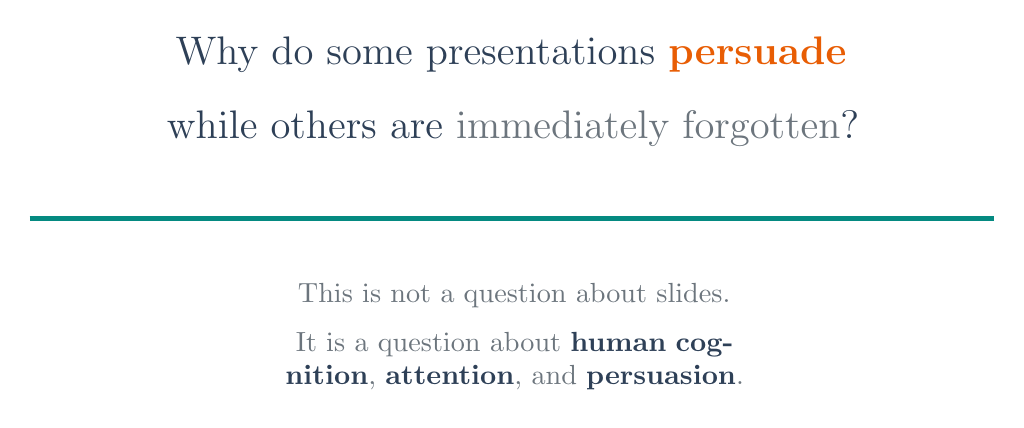
\begin{tikzpicture}
    % Large question
    \node[text=DeepNavy,font=\Large,text width=12cm,align=center] (q) {
        Why do some presentations \emphcolor{persuade}\\[0.3cm]
        while others are \graytext{immediately forgotten}?
    };

    % Visual separator
    \draw[Teal,line width=1.5pt] ([yshift=-0.8cm]q.south west) -- ([yshift=-0.8cm]q.south east);

    % Sub-points
    \node[below=1.5cm of q,text=WarmGray,font=\normalsize,text width=10cm,align=center] {
        This is not a question about slides.\\[0.2cm]
        It is a question about \textcolor{DeepNavy}{\textbf{human cognition}},
        \textcolor{DeepNavy}{\textbf{attention}}, and \textcolor{DeepNavy}{\textbf{persuasion}}.
    };
\end{tikzpicture}
\end{center}
\end{frame}

% -----------------------------------------------------------------------------
% SECTION: WHAT IS RHETORIC?
% -----------------------------------------------------------------------------
\transitionslide{Part I}{What Is Rhetoric?}

\begin{frame}
\frametitle{Rhetoric Is Not Ornament}
\vspace{0.3cm}

\begin{columns}[T]
\begin{column}{0.48\textwidth}
\textcolor{DeepRed}{\textbf{Common Misconception}}\\[0.3cm]
\graytext{Rhetoric as:}
\begin{itemize}
    \item Manipulation
    \item Empty flourish
    \item Style over substance
    \item ``Spin''
\end{itemize}
\end{column}

\begin{column}{0.48\textwidth}
\textcolor{Teal}{\textbf{What Rhetoric Actually Is}}\\[0.3cm]
The systematic study of \emphcolor{how humans persuade one another}
\vspace{0.4cm}

When communication succeeds, \textit{why}?\\
When it fails, \textit{why}?
\end{column}
\end{columns}

\vspace{0.8cm}
\begin{center}

\begin{tikzpicture}
\node[draw=Teal,rounded corners=3pt,inner sep=10pt,text=DeepNavy,fill=LightGray] {
    The same argument, presented differently, is \emphcolor{not the same argument}.
};
\end{tikzpicture}
\end{center}
\end{frame}

% -----------------------------------------------------------------------------
% ARISTOTLE'S FRAMEWORK
% -----------------------------------------------------------------------------
\begin{frame}
\frametitle{Aristotle's Framework}
\framesubtitle{Three modes of persuasion---still definitive after 2,400 years}
\vspace{0.3cm}

\begin{center}
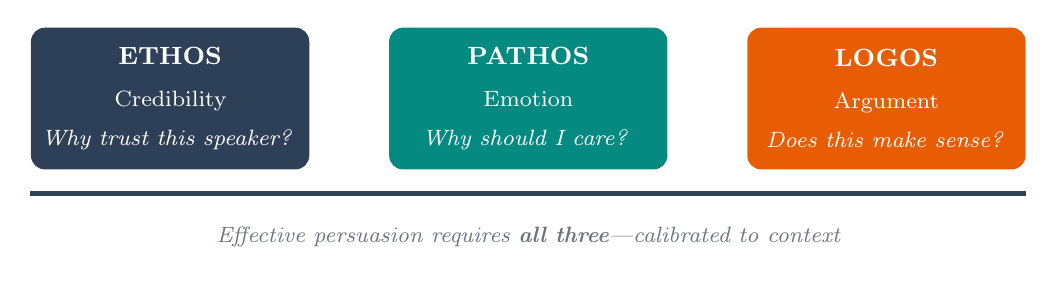
\begin{tikzpicture}[
    node distance=0.8cm,
    box/.style={rectangle, rounded corners=5pt, minimum width=3.5cm, minimum height=1.8cm,
                text centered, font=\small, text=white, text width=3.3cm, align=center}
]
    % Three pillars
    \node[box, fill=DeepNavy] (ethos) {\textbf{ETHOS}\\[0.2cm]\footnotesize Credibility\\[0.1cm]\textit{Why trust this speaker?}};
    \node[box, fill=Teal, right=1cm of ethos] (pathos) {\textbf{PATHOS}\\[0.2cm]\footnotesize Emotion\\[0.1cm]\textit{Why should I care?}};
    \node[box, fill=WarmOrange, right=1cm of pathos] (logos) {\textbf{LOGOS}\\[0.2cm]\footnotesize Argument\\[0.1cm]\textit{Does this make sense?}};

    % Connecting base
    \draw[DeepNavy, line width=2pt]
        ([yshift=-0.3cm]ethos.south west) -- ([yshift=-0.3cm]logos.south east);

    % Foundation label
    \node[below=0.6cm of pathos, text=WarmGray, font=\footnotesize\itshape] {
        Effective persuasion requires \textbf{all three}---calibrated to context
    };
\end{tikzpicture}
\end{center}
\end{frame}

% -----------------------------------------------------------------------------
% RHETORICAL TRADITION
% -----------------------------------------------------------------------------
\begin{frame}
\frametitle{A Continuous Tradition}
\vspace{0.2cm}

\begin{center}
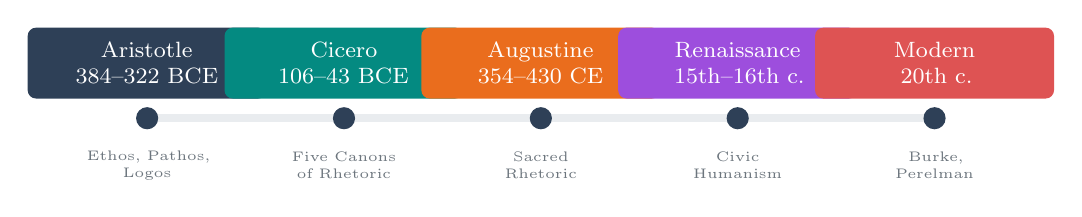
\begin{tikzpicture}[
    node distance=0.3cm,
    era/.style={rectangle, rounded corners=3pt, minimum height=0.9cm,
                text centered, font=\footnotesize, text=white, text width=2.8cm},
    label/.style={font=\tiny, text=WarmGray}
]
    % Timeline (aligned with first and last era boxes)
    \draw[LightGray, line width=3pt] (1,0) -- (11,0);

    % Era boxes
    \node[era, fill=DeepNavy] at (1,0.7) (aristotle) {Aristotle\\384--322 BCE};
    \node[era, fill=Teal] at (3.5,0.7) (cicero) {Cicero\\106--43 BCE};
    \node[era, fill=WarmOrange!90] at (6,0.7) (augustine) {Augustine\\354--430 CE};
    \node[era, fill=SoftPurple] at (8.5,0.7) (renaissance) {Renaissance\\15th--16th c.};
    \node[era, fill=DeepRed!80] at (11,0.7) (modern) {Modern\\20th c.};

    % Contributions (below)
    \node[label, text width=2.5cm, align=center] at (1,-0.6) {Ethos, Pathos,\\Logos};
    \node[label, text width=2.5cm, align=center] at (3.5,-0.6) {Five Canons\\of Rhetoric};
    \node[label, text width=2.5cm, align=center] at (6,-0.6) {Sacred\\Rhetoric};
    \node[label, text width=2.5cm, align=center] at (8.5,-0.6) {Civic\\Humanism};
    \node[label, text width=2.5cm, align=center] at (11,-0.6) {Burke,\\Perelman};

    % Timeline dots
    \foreach \x in {1,3.5,6,8.5,11} {
        \fill[DeepNavy] (\x,0) circle (4pt);
    }
\end{tikzpicture}
\end{center}

\vspace{0.5cm}
\begin{center}
\graytext{\small The core questions persist: How does communication persuade?}
\end{center}
\end{frame}

% -----------------------------------------------------------------------------
% SECTION: TECHNOLOGY
% -----------------------------------------------------------------------------
\transitionslide{Part II}{Technology Changes the Medium,\\Not the Principles}

\begin{frame}
\frametitle{Each Era Transforms the Rhetorical Situation}
\vspace{0.2cm}

\begin{center}
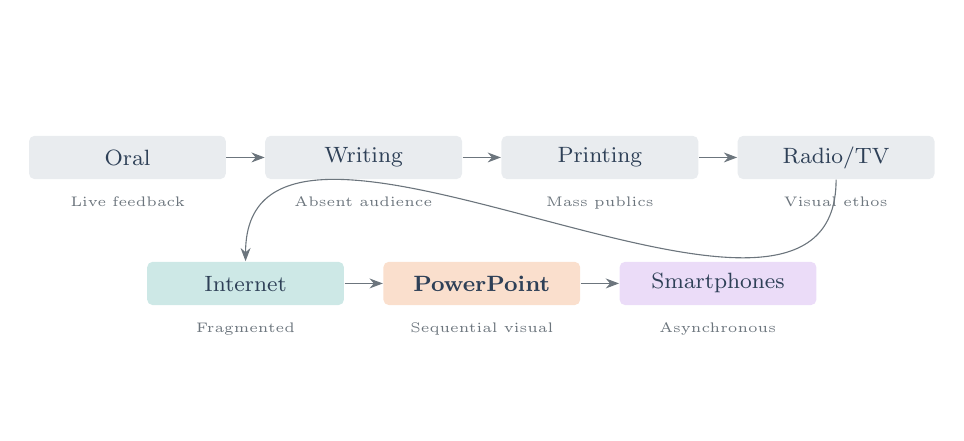
\begin{tikzpicture}[
    node distance=0.4cm,
    tech/.style={rectangle, rounded corners=2pt, minimum height=0.55cm,
                 text centered, font=\footnotesize, fill=LightGray, text=DeepNavy,
                 minimum width=2.5cm},
    impact/.style={font=\tiny, text=WarmGray, text width=2.3cm, align=center}
]
    % Technologies - scaled down
    \node[tech] (oral) at (0,2.5) {Oral};
    \node[tech] (writing) at (3,2.5) {Writing};
    \node[tech] (print) at (6,2.5) {Printing};
    \node[tech] (broadcast) at (9,2.5) {Radio/TV};

    \node[tech, fill=Teal!20] (internet) at (1.5,0.9) {Internet};
    \node[tech, fill=WarmOrange!20] (ppt) at (4.5,0.9) {\textbf{PowerPoint}};
    \node[tech, fill=SoftPurple!20] (phone) at (7.5,0.9) {Smartphones};

    % Arrows showing progression
    \draw[-{Stealth}, WarmGray] (oral) -- (writing);
    \draw[-{Stealth}, WarmGray] (writing) -- (print);
    \draw[-{Stealth}, WarmGray] (print) -- (broadcast);

    \draw[-{Stealth}, WarmGray] (broadcast.south) to[out=-90,in=90] (internet.north);
    \draw[-{Stealth}, WarmGray] (internet) -- (ppt);
    \draw[-{Stealth}, WarmGray] (ppt) -- (phone);

    % Impact labels
    \node[impact, below=0.1cm of oral] {Live feedback};
    \node[impact, below=0.1cm of writing] {Absent audience};
    \node[impact, below=0.1cm of print] {Mass publics};
    \node[impact, below=0.1cm of broadcast] {Visual ethos};

    \node[impact, below=0.1cm of internet] {Fragmented};
    \node[impact, below=0.1cm of ppt] {Sequential visual};
    \node[impact, below=0.1cm of phone] {Asynchronous};
\end{tikzpicture}
\end{center}
\end{frame}

\begin{frame}
\frametitle{And Then PowerPoint}
\framesubtitle{1987---A new medium, rarely theorized}
\vspace{0.5cm}

\begin{columns}[T]
\begin{column}{0.55\textwidth}
Slide decks became \emphcolor{ubiquitous}:
\begin{itemize}
    \item Business
    \item Education
    \item Government
    \item Military
\end{itemize}

\vspace{0.5cm}
They structure how organizations \textbf{think}, \textbf{decide}, and \textbf{communicate}.

\vspace{0.5cm}
\graytext{\footnotesize Hundreds of millions of presentations daily.}
\end{column}

\begin{column}{0.4\textwidth}
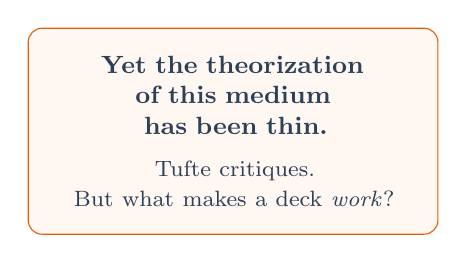
\begin{tikzpicture}
    \node[draw=WarmOrange, rounded corners=5pt, inner sep=10pt,
          text=DeepNavy, text width=4.5cm, align=center, fill=WarmOrange!5, font=\small] {
        \textbf{Yet the theorization\\of this medium\\has been thin.}\\[0.2cm]
        \footnotesize Tufte critiques.\\
        But what makes a deck \textit{work}?
    };
\end{tikzpicture}
\end{column}
\end{columns}
\end{frame}

% -----------------------------------------------------------------------------
% SECTION: WHAT IS A DECK?
% -----------------------------------------------------------------------------
\transitionslide{Part III}{What Is a Deck?}

\begin{frame}
\frametitle{Definition}
\vspace{0.3cm}

\begin{center}

\begin{tikzpicture}
    \node[text=DeepNavy, font=\large, text width=11cm, align=center] (def) {
        A slide deck is a form of\\[0.15cm]
        \emphcolor{sequential visual rhetoric}\\[0.15cm]
        designed to accompany spoken argument.
    };
\end{tikzpicture}
\end{center}

\vspace{0.5cm}

\begin{columns}[T]
\begin{column}{0.24\textwidth}
\centering
\textcolor{Teal}{\textbf{Sequential}}\\[0.15cm]
\scriptsize Ordered. Slide 1 precedes Slide 2. Inherently \textit{narrative}.
\end{column}
\begin{column}{0.24\textwidth}
\centering
\textcolor{Teal}{\textbf{Visual}}\\[0.15cm]
\scriptsize Composition, not text. The channel matters.
\end{column}
\begin{column}{0.24\textwidth}
\centering
\textcolor{Teal}{\textbf{Rhetoric}}\\[0.15cm]
\scriptsize Aims to persuade. Ethos, pathos, logos apply.
\end{column}
\begin{column}{0.24\textwidth}
\centering
\textcolor{Teal}{\textbf{Accompaniment}}\\[0.15cm]
\scriptsize \emphcolor{Not} a document. Serves the speaker.
\end{column}
\end{columns}
\end{frame}

\begin{frame}
\frametitle{The Analogy to Comics}
\framesubtitle{Scott McCloud's insight about sequential art}
\vspace{0.1cm}

\begin{center}
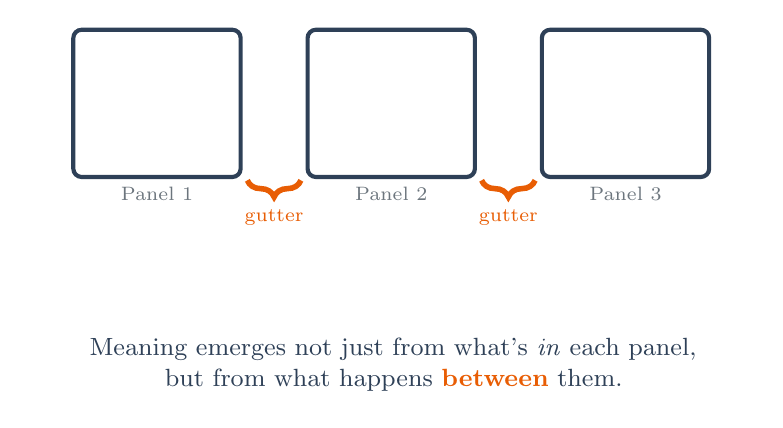
\begin{tikzpicture}[scale=0.85]
    % Three panels representing comic frames
    \foreach \i/\label in {0/Panel 1, 3.5/Panel 2, 7/Panel 3} {
        \draw[DeepNavy, line width=1.5pt, rounded corners=3pt]
            (\i,0) rectangle (\i+2.5,2.2);
        \node[font=\scriptsize, text=WarmGray] at (\i+1.25, -0.25) {\label};
    }

    % The "gutter" annotations
    \draw[WarmOrange, line width=2pt, decorate, decoration={brace, amplitude=6pt, mirror}]
        (2.6, -0.05) -- (3.4, -0.05);
    \draw[WarmOrange, line width=2pt, decorate, decoration={brace, amplitude=6pt, mirror}]
        (6.1, -0.05) -- (6.9, -0.05);

    \node[font=\scriptsize, text=WarmOrange] at (3, -0.6) {gutter};
    \node[font=\scriptsize, text=WarmOrange] at (6.5, -0.6) {gutter};

    % Key insight
    \node[below=1.2cm of current bounding box.south, text=DeepNavy, font=\small,
          text width=9cm, align=center] {
        Meaning emerges not just from what's \textit{in} each panel,\\
        but from what happens \emphcolor{between} them.
    };
\end{tikzpicture}
\end{center}

\vspace{0.3cm}
\begin{center}
\graytext{\small Decks work similarly: transitions, juxtaposition, progressive revelation.}
\end{center}
\end{frame}

% -----------------------------------------------------------------------------
% SECTION: AESTHETICS
% -----------------------------------------------------------------------------
\transitionslide{Part IV}{Why Beauty Matters}

\begin{frame}
\frametitle{The Economics of Attention}
\vspace{0.1cm}

\begin{center}
\begin{tikzpicture}[scale=0.85, every node/.style={scale=0.85}]
    % Central person icon
    \node[circle, fill=DeepNavy, minimum size=1cm, text=white, font=\normalsize] (person) {\faUser};

    % Competing demands
    \node[right=1.6cm of person, text=DeepRed, font=\footnotesize] (phone) {\faPhone~Phone};
    \node[above right=0.9cm and 1.2cm of person, text=WarmGray, font=\footnotesize] (email) {\faEnvelope~Email};
    \node[below right=0.9cm and 1.2cm of person, text=WarmGray, font=\footnotesize] (meeting) {\faCalendar~Meeting};
    \node[above=1.4cm of person, text=WarmGray, font=\footnotesize] (worry) {\faBrain~Worries};
    \node[below=1.4cm of person, text=WarmGray, font=\footnotesize] (last) {\faArrowLeft~Last slide};

    % Arrows pointing at person
    \draw[-{Stealth}, WarmGray, thick] (phone) -- (person);
    \draw[-{Stealth}, WarmGray] (email) -- (person);
    \draw[-{Stealth}, WarmGray] (meeting) -- (person);
    \draw[-{Stealth}, WarmGray] (worry) -- (person);
    \draw[-{Stealth}, WarmGray] (last) -- (person);

    % Your slide competing
    \node[left=2cm of person, draw=Teal, rounded corners=3pt,
          inner sep=6pt, text=Teal, font=\footnotesize\bfseries] (slide) {Your Slide};
    \draw[-{Stealth}, Teal, very thick] (slide) -- (person);
\end{tikzpicture}
\end{center}

\vspace{0.3cm}
\begin{center}

\begin{tikzpicture}
\node[draw=WarmOrange, rounded corners=3pt, inner sep=8pt, text=DeepNavy, fill=WarmOrange!5, font=\small] {
    Attention is not \textbf{given}. It is \emphcolor{won}---slide by slide, moment by moment.
};
\end{tikzpicture}
\end{center}
\end{frame}

\begin{frame}
\frametitle{The Netflix Phenomenology}
\framesubtitle{Theater vs. streaming---and what it means for presentations}
\vspace{0.3cm}

\begin{columns}[T]
\begin{column}{0.45\textwidth}
\textcolor{Teal}{\textbf{Theater}}\\[0.3cm]
\begin{itemize}
    \item Captive audience
    \item Social norms enforce attention
    \item Phone use conspicuous
    \item Invested (paid, traveled)
\end{itemize}

\vspace{0.3cm}
\graytext{\footnotesize Kurosawa, Leone, Scorsese could trust sustained attention.}
\end{column}

\begin{column}{0.45\textwidth}
\textcolor{WarmOrange}{\textbf{Streaming (and Presentations)}}\\[0.3cm]
\begin{itemize}
    \item Contestable attention
    \item Distractions everywhere
    \item Pausing effortless
    \item Minds wander
\end{itemize}

\vspace{0.3cm}
\graytext{\footnotesize Netflix advised: \textit{regularly remind viewers of the plot}.}
\end{column}
\end{columns}

\vspace{0.5cm}
\begin{center}
\emphcolor{A presentation faces conditions closer to streaming than theater.}
\end{center}
\end{frame}

\begin{frame}
\frametitle{Why Beauty Draws}
\vspace{0.1cm}

\begin{center}
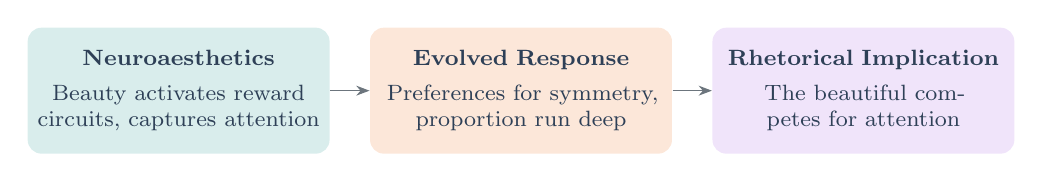
\begin{tikzpicture}[
    box/.style={rectangle, rounded corners=5pt, minimum width=3.8cm, minimum height=1.6cm,
                text centered, font=\footnotesize, text=DeepNavy, text width=3.6cm, align=center}
]
    % Neuroaesthetics finding
    \node[box, fill=Teal!15] (neuro) at (0,0) {
        \textbf{Neuroaesthetics}\\[0.1cm]
        Beauty activates reward circuits, captures attention
    };

    % Evolutionary account
    \node[box, fill=WarmOrange!15, right=0.5cm of neuro] (evo) {
        \textbf{Evolved Response}\\[0.1cm]
        Preferences for symmetry, proportion run deep
    };

    % Implication
    \node[box, fill=SoftPurple!15, right=0.5cm of evo] (impl) {
        \textbf{Rhetorical Implication}\\[0.1cm]
        The beautiful competes for attention
    };

    % Arrows
    \draw[-{Stealth}, WarmGray] (neuro) -- (evo);
    \draw[-{Stealth}, WarmGray] (evo) -- (impl);
\end{tikzpicture}
\end{center}

\vspace{0.4cm}
\begin{center}

\begin{tikzpicture}
\node[text=DeepNavy, font=\normalsize, text width=10cm, align=center] {
    A beautiful slide says, without saying:\\[0.15cm]
    \emphcolor{\textit{This is worth looking at.}}
};
\end{tikzpicture}
\end{center}
\end{frame}

\begin{frame}
\frametitle{Aesthetics as Ethics}
\vspace{0.1cm}

\begin{center}
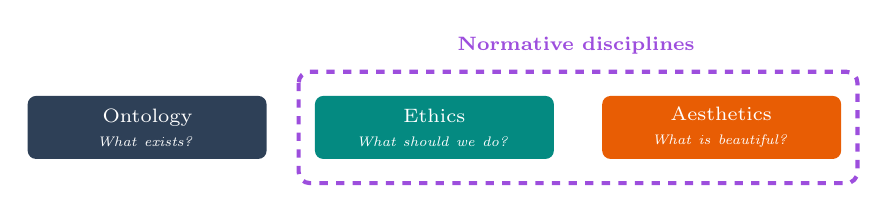
\begin{tikzpicture}[
    node distance=0.3cm,
    branch/.style={rectangle, rounded corners=3pt, minimum height=0.8cm,
                   text centered, font=\scriptsize, text=white, text width=2.8cm}
]
    % Philosophy branches
    \node[branch, fill=DeepNavy] (onto) {Ontology\\[0.02cm]\tiny\textit{What exists?}};
    \node[branch, fill=Teal, right=0.6cm of onto] (ethics) {Ethics\\[0.02cm]\tiny\textit{What should we do?}};
    \node[branch, fill=WarmOrange, right=0.6cm of ethics] (aesthetics) {Aesthetics\\[0.02cm]\tiny\textit{What is beautiful?}};

    % Grouping
    \draw[SoftPurple, line width=1.5pt, rounded corners=4pt, dashed]
        ([xshift=-0.2cm, yshift=0.3cm]ethics.north west) rectangle
        ([xshift=0.2cm, yshift=-0.3cm]aesthetics.south east);

    \node[above=0.4cm of ethics, xshift=1.8cm, text=SoftPurple, font=\scriptsize\bfseries] {Normative disciplines};
\end{tikzpicture}
\end{center}

\vspace{0.4cm}

\begin{columns}[T]
\begin{column}{0.58\textwidth}
\footnotesize
The presenter who takes the audience's time \emphcolor{owes them something}:

\vspace{0.2cm}
Not merely information, but information \textit{rendered well}.

\vspace{0.2cm}
To present ugly slides is a form of disrespect.
\end{column}
\begin{column}{0.38\textwidth}
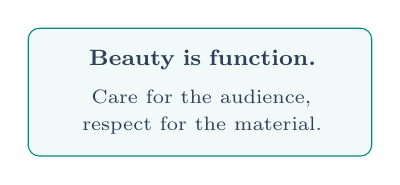
\begin{tikzpicture}
\node[draw=Teal, rounded corners=4pt, inner sep=8pt, text=DeepNavy,
      text width=3.8cm, align=center, fill=Teal!5, font=\footnotesize] {
    \textbf{Beauty is function.}\\[0.15cm]
    \scriptsize Care for the audience, respect for the material.
};
\end{tikzpicture}
\end{column}
\end{columns}
\end{frame}

% -----------------------------------------------------------------------------
% SHKLOVSKY
% -----------------------------------------------------------------------------
\begin{frame}
\frametitle{Defamiliarization}
\framesubtitle{Viktor Shklovsky, 1917: Making the stones feel like stones}
\vspace{0.05cm}

\begin{center}
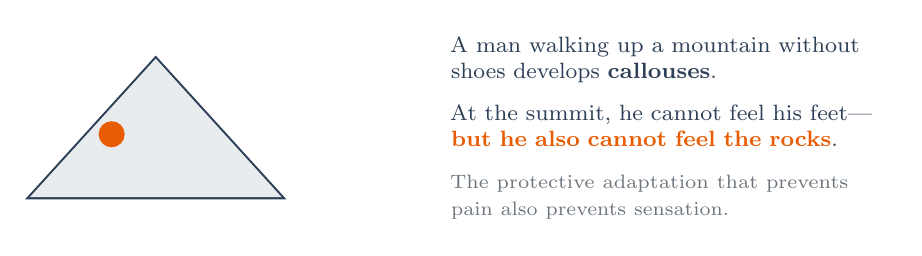
\begin{tikzpicture}[scale=0.8]
    % Mountain illustration
    \draw[DeepNavy, line width=1.5pt]
        (0,0) -- (2,2.2) -- (4,0) -- cycle;
    \fill[LightGray] (0,0) -- (2,2.2) -- (4,0) -- cycle;

    % Person walking up
    \node[circle, fill=WarmOrange, minimum size=0.3cm] at (1.3, 1.0) {};

    % Callouses metaphor
    \node[right=2cm of current bounding box.east, text=DeepNavy, font=\footnotesize,
          text width=5.5cm, align=left] {
        A man walking up a mountain without shoes develops \textbf{callouses}.\\[0.2cm]
        At the summit, he cannot feel his feet---\emphcolor{but he also cannot feel the rocks}.\\[0.2cm]
        \graytext{\scriptsize The protective adaptation that prevents pain also prevents sensation.}
    };
\end{tikzpicture}
\end{center}

\vspace{0.15cm}
\begin{center}

\begin{tikzpicture}
\node[draw=Teal, rounded corners=3pt, inner sep=8pt, text=DeepNavy, fill=Teal!5,
      text width=9cm, align=center, font=\footnotesize] {
    \textbf{Art exists to restore sensation.}
    The effective deck must make the stones feel like stones again.
};
\end{tikzpicture}
\end{center}
\end{frame}

\begin{frame}
\frametitle{How to Defamiliarize}
\vspace{0.2cm}

\begin{columns}[T]
\begin{column}{0.48\textwidth}
\textcolor{Teal}{\textbf{Techniques}}\\[0.3cm]

\textbf{The unexpected visual}\\
\graytext{\footnotesize Figure where bullets expected.}

\vspace{0.3cm}
\textbf{Provocative framing}\\
\graytext{\footnotesize Not ``Sales up 15\%'' but ``A 737's worth of revenue weekly.''}

\vspace{0.3cm}
\textbf{Violation of expectation}\\
\graytext{\footnotesize Devil's Advocate slide. Conclusion before evidence.}
\end{column}

\begin{column}{0.48\textwidth}
\textcolor{WarmOrange}{\textbf{The Goal}}\\[0.3cm]

Break the trance of habitual reception.

\vspace{0.2cm}
Pull the audience out of their phones.

\vspace{0.2cm}
Demand \emphcolor{genuine cognitive engagement}.

\vspace{0.3cm}
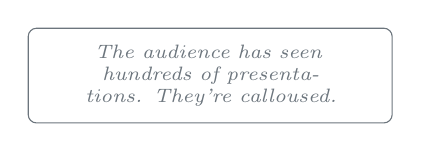
\begin{tikzpicture}
\node[draw=WarmGray, rounded corners=3pt, inner sep=6pt, text=WarmGray,
      text width=4.2cm, align=center, font=\scriptsize\itshape] {
    The audience has seen hundreds of presentations. They're calloused.
};
\end{tikzpicture}
\end{column}
\end{columns}
\end{frame}

% -----------------------------------------------------------------------------
% SECTION: FIRST PRINCIPLES
% -----------------------------------------------------------------------------
\transitionslide{Part V}{First Principles}

\begin{frame}
\frametitle{The Law of Cognitive Load}

\begin{center}
\begin{tikzpicture}[scale=0.8]
    % Brain with limited capacity
    \node[circle, fill=DeepNavy!10, minimum size=2.3cm,
          draw=DeepNavy, line width=1.5pt] (brain) {};
    \node[text=DeepNavy, font=\normalsize] at (brain.center) {\faBrain};

    % Limited capacity indicator
    \draw[WarmOrange, line width=2pt]
        ([xshift=-0.5cm, yshift=-1.4cm]brain.center) --
        ([xshift=0.5cm, yshift=-1.4cm]brain.center);
    \node[below=1.6cm of brain, text=WarmOrange, font=\scriptsize\bfseries] {Limited Working Memory};

    % Input arrows (too many)
    \foreach \angle in {150, 120, 90, 60, 30} {
        \draw[-{Stealth}, WarmGray]
            ([shift={(\angle:2cm)}]brain.center) -- ([shift={(\angle:1.3cm)}]brain.center);
    }

    % Key insight
    \node[right=2.5cm of brain, text=DeepNavy, font=\footnotesize,
          text width=5.5cm, align=left] {
        Every element consumes cognitive resources.\\[0.2cm]
        When resources are exhausted, \emphcolor{comprehension fails}.\\[0.2cm]
        \graytext{\scriptsize A slide with 3 bullet points $\times$ 12 words each may produce \textit{less} understanding than one clear point.}
    };
\end{tikzpicture}
\end{center}

\vspace{0.1cm}
\begin{center}
\normalsize\color{DeepNavy}\textbf{One idea per slide. One.}
\end{center}
\end{frame}

\begin{frame}
\frametitle{The Marginal Principle}
\framesubtitle{Smoothness as default, surprise as intention}
\vspace{0.1cm}

\begin{center}
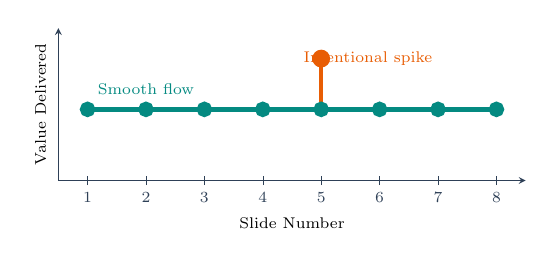
\begin{tikzpicture}[scale=0.8]
    \begin{axis}[
        width=9cm, height=4cm,
        xlabel={Slide Number},
        ylabel={Value Delivered},
        xlabel style={font=\scriptsize},
        ylabel style={font=\scriptsize},
        xtick={1,2,3,4,5,6,7,8},
        ytick=\empty,
        xmin=0.5, xmax=8.5,
        ymin=0, ymax=1.5,
        axis lines=left,
        axis line style={DeepNavy},
        tick style={DeepNavy},
        ticklabel style={font=\scriptsize, text=DeepNavy}
    ]
    % Baseline smooth flow
    \addplot[Teal, line width=2pt, mark=*, mark size=2.5pt]
        coordinates {(1,0.7) (2,0.7) (3,0.7) (4,0.7) (5,0.7) (6,0.7) (7,0.7) (8,0.7)};

    % Surprise spike
    \addplot[WarmOrange, line width=2pt, mark=*, mark size=3pt, only marks]
        coordinates {(5,1.2)};
    \draw[WarmOrange, line width=2pt] (axis cs:5,0.7) -- (axis cs:5,1.2);

    \node[font=\scriptsize, text=Teal] at (axis cs:2,0.9) {Smooth flow};
    \node[font=\scriptsize, text=WarmOrange] at (axis cs:5.8,1.2) {Intentional spike};
    \end{axis}
\end{tikzpicture}
\end{center}

\vspace{0.15cm}
\begin{columns}[T]
\begin{column}{0.48\textwidth}
\textcolor{Teal}{\textbf{Smoothness}}\\
\graytext{\scriptsize Equal marginal benefit per unit of attention. The audience develops a rhythm.}
\end{column}
\begin{column}{0.48\textwidth}
\textcolor{WarmOrange}{\textbf{Surprise}}\\
\graytext{\scriptsize Break the rhythm when it matters. The core finding. The devastating question.}
\end{column}
\end{columns}
\end{frame}

\begin{frame}
\frametitle{The Slide Serves the Spoken Word}
\vspace{0.3cm}

\begin{center}
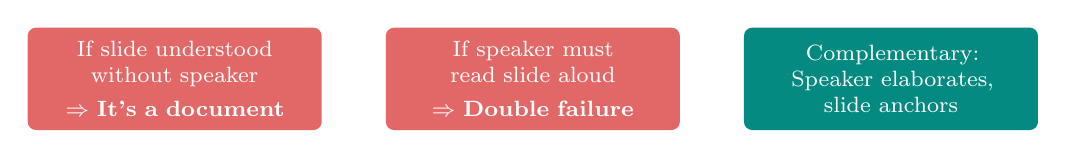
\begin{tikzpicture}[
    node distance=0.7cm,
    box/.style={rectangle, rounded corners=3pt, minimum height=1.3cm,
                text centered, font=\footnotesize, text=white, text width=3.5cm}
]
    % Test 1
    \node[box, fill=DeepRed!70] (test1) {
        If slide understood\\without speaker\\[0.1cm]
        $\Rightarrow$ \textbf{It's a document}
    };

    % Test 2
    \node[box, fill=DeepRed!70, right=0.8cm of test1] (test2) {
        If speaker must\\read slide aloud\\[0.1cm]
        $\Rightarrow$ \textbf{Double failure}
    };

    % Right answer
    \node[box, fill=Teal, right=0.8cm of test2] (right) {
        Complementary:\\Speaker elaborates,\\slide anchors
    };
\end{tikzpicture}
\end{center}

\vspace{0.5cm}
\begin{center}
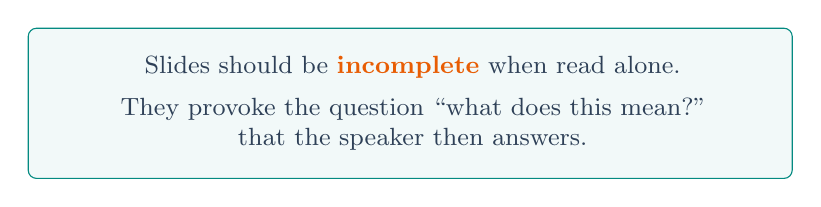
\begin{tikzpicture}
\node[draw=Teal, rounded corners=3pt, inner sep=10pt, text=DeepNavy, fill=Teal!5,
      text width=9cm, align=center, font=\small] {
    Slides should be \emphcolor{incomplete} when read alone.\\[0.15cm]
    They provoke the question ``what does this mean?''\\
    that the speaker then answers.
};
\end{tikzpicture}
\end{center}
\end{frame}

% -----------------------------------------------------------------------------
% REMINDING THE PLOT
% -----------------------------------------------------------------------------
\begin{frame}
\frametitle{Reminding Them of the Plot}
\framesubtitle{Bad ways vs. good ways}
\vspace{0.2cm}

\begin{columns}[T]
\begin{column}{0.45\textwidth}
\textcolor{DeepRed}{\textbf{Bad Reminders}}\\[0.3cm]

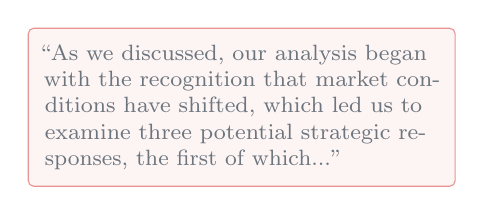
\begin{tikzpicture}
\node[draw=DeepRed!50, rounded corners=2pt, inner sep=6pt,
      text=WarmGray, font=\footnotesize, text width=5cm, fill=DeepRed!5] {
    ``As we discussed, our analysis began with the recognition that market conditions have shifted, which led us to examine three potential strategic responses, the first of which...''
};
\end{tikzpicture}

\vspace{0.3cm}
\graytext{\footnotesize\faTimesCircle\hspace{0.2cm}Verbose recap}

\vspace{0.2cm}
\graytext{\footnotesize\faTimesCircle\hspace{0.2cm}Identical repetition}

\vspace{0.2cm}
\graytext{\footnotesize\faTimesCircle\hspace{0.2cm}``In case anyone wasn't paying attention...''}

\vspace{0.2cm}
\graytext{\footnotesize\faTimesCircle\hspace{0.2cm}Agenda slide ad nauseam}
\end{column}

\begin{column}{0.45\textwidth}
\textcolor{Teal}{\textbf{Good Reminders}}\\[0.3cm]

\tealtext{\footnotesize\faCheckCircle\hspace{0.2cm}Structural markers}\\
\graytext{\tiny Brief visual cues showing location in argument}

\vspace{0.25cm}
\tealtext{\footnotesize\faCheckCircle\hspace{0.2cm}Backward link in forward claim}\\
\graytext{\tiny ``This 15\% gain we identified earlier compounds when...''}

\vspace{0.25cm}
\tealtext{\footnotesize\faCheckCircle\hspace{0.2cm}Visual callbacks}\\
\graytext{\tiny Earlier figure, now with new annotation}

\vspace{0.25cm}
\tealtext{\footnotesize\faCheckCircle\hspace{0.2cm}Titles that orient}\\
\graytext{\tiny ``Robustness Check 3'' not just ``Analysis''}
\end{column}
\end{columns}
\end{frame}

% -----------------------------------------------------------------------------
% SECTION: LLMs
% -----------------------------------------------------------------------------
\transitionslide{Part VI}{Large Language Models\\and Tacit Knowledge}

\begin{frame}
\frametitle{The Jagged Frontier}
\framesubtitle{David Autor's insight about AI and labor}
\vspace{0.3cm}

\begin{center}
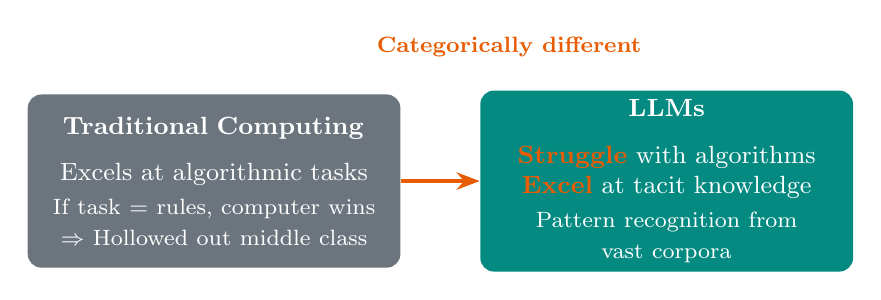
\begin{tikzpicture}[
    box/.style={rectangle, rounded corners=5pt, minimum height=2.2cm,
                text centered, font=\small, text=white, text width=4.5cm}
]
    % Traditional computers
    \node[box, fill=WarmGray] (trad) {
        \textbf{Traditional Computing}\\[0.2cm]
        Excels at algorithmic tasks\\[0.1cm]
        \footnotesize If task = rules, computer wins\\
        $\Rightarrow$ Hollowed out middle class
    };

    % LLMs
    \node[box, fill=Teal, right=1cm of trad] (llm) {
        \textbf{LLMs}\\[0.2cm]
        \emphcolor{Struggle} with algorithms\\
        \emphcolor{Excel} at tacit knowledge\\[0.1cm]
        \footnotesize Pattern recognition from\\vast corpora
    };

    % Arrow
    \draw[-{Stealth}, WarmOrange, very thick] (trad) -- (llm);
    \node[above=0.3cm of llm, xshift=-2cm, text=WarmOrange, font=\footnotesize\bfseries] {Categorically different};
\end{tikzpicture}
\end{center}

\vspace{0.5cm}
\begin{center}
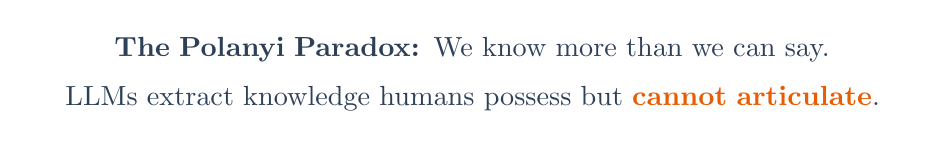
\begin{tikzpicture}
\node[text=DeepNavy, font=\normalsize, text width=11cm, align=center] {
    \textbf{The Polanyi Paradox:} We know more than we can say.\\[0.2cm]
    LLMs extract knowledge humans possess but \emphcolor{cannot articulate}.
};
\end{tikzpicture}
\end{center}
\end{frame}

\begin{frame}
\frametitle{What LLMs Have Seen}
\vspace{0.1cm}

\begin{columns}[T]
\begin{column}{0.55\textwidth}
\footnotesize
Trained on materials including:
\begin{itemize}
    \setlength{\itemsep}{1pt}
    \item Countless slide decks
    \item Presentation outlines
    \item Books on communication
    \item Research on cognition
\end{itemize}

\vspace{0.2cm}
But also seemingly unrelated:
\begin{itemize}
    \setlength{\itemsep}{1pt}
    \item Mad Magazine's visual satire
    \item Sports Illustrated's data narrative
    \item Stereo manuals' technical clarity
    \item TV Guide's compression
\end{itemize}
\end{column}

\begin{column}{0.4\textwidth}
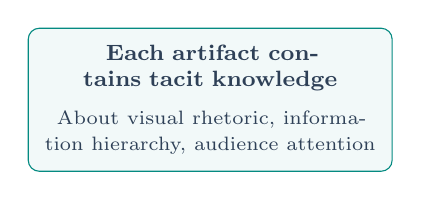
\begin{tikzpicture}
\node[draw=Teal, rounded corners=4pt, inner sep=6pt, text=DeepNavy,
      text width=4.2cm, align=center, fill=Teal!5, font=\footnotesize] {
    \textbf{Each artifact contains tacit knowledge}\\[0.15cm]
    \scriptsize About visual rhetoric,
    information hierarchy,
    audience attention
};
\end{tikzpicture}
\end{column}
\end{columns}

\vspace{0.2cm}
\begin{center}
\graytext{\scriptsize LLMs develop sensitivities to what works---across more examples than any human encounters.}
\end{center}
\end{frame}

% -----------------------------------------------------------------------------
% SECTION: CASE STUDY
% -----------------------------------------------------------------------------
\transitionslide{Part VII}{Case Study:\\The Academic Job Market Talk}

\begin{frame}
\frametitle{The Stakes}
\vspace{0.5cm}

\begin{center}
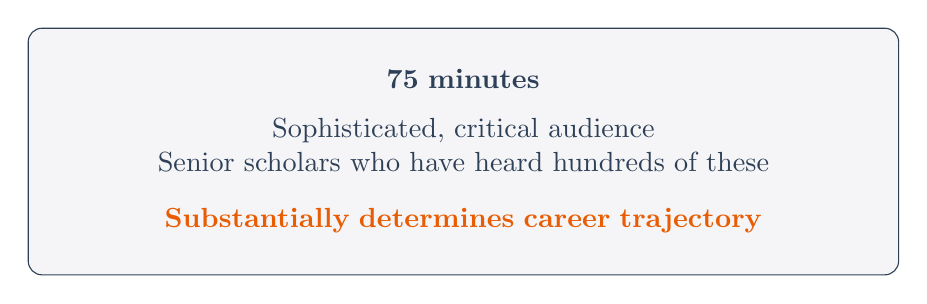
\begin{tikzpicture}
    % Context box
    \node[draw=DeepNavy, rounded corners=5pt, inner sep=15pt, text=DeepNavy,
          text width=10cm, align=center, fill=DeepNavy!5] {
        \textbf{75 minutes}\\[0.2cm]
        Sophisticated, critical audience\\
        Senior scholars who have heard hundreds of these\\[0.3cm]
        \emphcolor{Substantially determines career trajectory}
    };
\end{tikzpicture}
\end{center}

\vspace{0.8cm}
\begin{center}
\Large\color{DeepNavy}
This context demands the \emphcolor{full apparatus}\\of deck rhetoric.
\end{center}
\end{frame}

\begin{frame}
\frametitle{The First Slide: Establishing the Plot}
\framesubtitle{Bad vs. Good}
\vspace{0.2cm}

\begin{columns}[T]
\begin{column}{0.45\textwidth}
\textcolor{DeepRed}{\textbf{Bad First Slide}}\\[0.3cm]

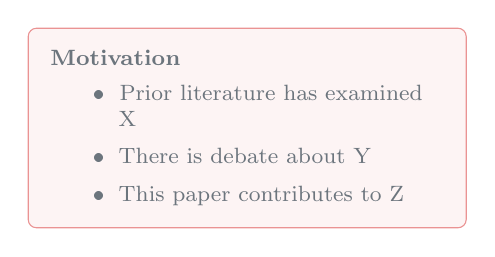
\begin{tikzpicture}
\node[draw=DeepRed!50, rounded corners=3pt, inner sep=8pt,
      text=WarmGray, font=\footnotesize, text width=5cm, fill=DeepRed!5] {
    \textbf{Motivation}
    \begin{itemize}
        \setlength{\itemsep}{2pt}
        \item Prior literature has examined X
        \item There is debate about Y
        \item This paper contributes to Z
    \end{itemize}
};
\end{tikzpicture}

\vspace{0.3cm}
\graytext{\footnotesize Generic. Bloodless.\\Could describe any paper.}
\end{column}

\begin{column}{0.45\textwidth}
\textcolor{Teal}{\textbf{Good First Slide}}\\[0.3cm]

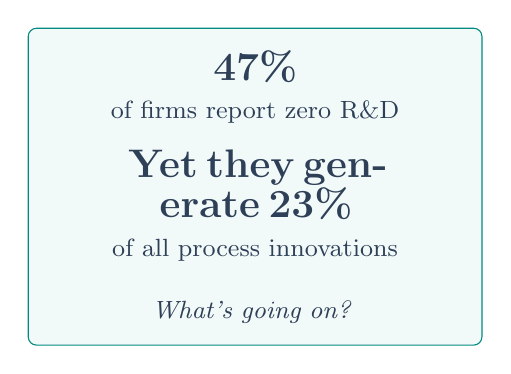
\begin{tikzpicture}
\node[draw=Teal, rounded corners=3pt, inner sep=8pt,
      text=DeepNavy, font=\small, text width=5.2cm, fill=Teal!5, align=center] {
    {\Large\bfseries 47\%}\\[0.1cm]
    of firms report zero R\&D\\[0.3cm]
    {\Large\bfseries Yet they generate 23\%}\\[0.1cm]
    of all process innovations\\[0.4cm]
    \textit{What's going on?}
};
\end{tikzpicture}

\vspace{0.3cm}
\tealtext{\footnotesize Creates a puzzle. Audience curious.\\Plot established.}
\end{column}
\end{columns}
\end{frame}

\begin{frame}
\frametitle{The Methodology Slide: Ethos Through Transparency}
\vspace{0.2cm}

\begin{columns}[T]
\begin{column}{0.45\textwidth}
\textcolor{DeepRed}{\textbf{Bad: Hides Behind Jargon}}\\[0.3cm]

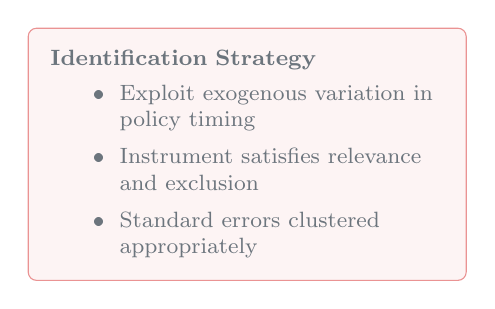
\begin{tikzpicture}
\node[draw=DeepRed!50, rounded corners=3pt, inner sep=8pt,
      text=WarmGray, font=\footnotesize, text width=5cm, fill=DeepRed!5] {
    \textbf{Identification Strategy}
    \begin{itemize}
        \setlength{\itemsep}{2pt}
        \item Exploit exogenous variation in policy timing
        \item Instrument satisfies relevance and exclusion
        \item Standard errors clustered appropriately
    \end{itemize}
};
\end{tikzpicture}

\vspace{0.2cm}
\graytext{\footnotesize Asserts without demonstrating.}
\end{column}

\begin{column}{0.48\textwidth}
\textcolor{Teal}{\textbf{Good: Shows the Work}}\\[0.3cm]

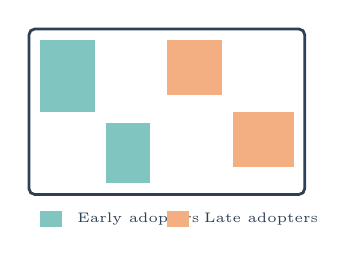
\begin{tikzpicture}[scale=0.7]
    % Simple map visualization
    \draw[DeepNavy, line width=1pt, rounded corners=2pt] (0,0) rectangle (5,3);

    % States (simplified)
    \fill[Teal!50] (0.2,1.5) rectangle (1.2,2.8);
    \fill[Teal!50] (1.4,0.2) rectangle (2.2,1.3);
    \fill[WarmOrange!50] (2.5,1.8) rectangle (3.5,2.8);
    \fill[WarmOrange!50] (3.7,0.5) rectangle (4.8,1.5);

    % Legend
    \fill[Teal!50] (0.2,-0.6) rectangle (0.6,-0.3);
    \node[right, font=\tiny, text=DeepNavy] at (0.7,-0.45) {Early adopters};
    \fill[WarmOrange!50] (2.5,-0.6) rectangle (2.9,-0.3);
    \node[right, font=\tiny, text=DeepNavy] at (3,-0.45) {Late adopters};
\end{tikzpicture}

\vspace{0.2cm}
\graytext{\footnotesize\textit{Policy rolled out state-by-state, 2003-2011.\\We compare early vs.\ late, before vs.\ after.}}

\vspace{0.2cm}
\tealtext{\footnotesize Audience can \textbf{see} the variation.}
\end{column}
\end{columns}
\end{frame}

% -----------------------------------------------------------------------------
% EXAMPLE FIGURES FROM R
% -----------------------------------------------------------------------------
\begin{frame}
\frametitle{Example: The College Wage Premium}
\framesubtitle{A century of skill-biased technological change}

\begin{center}
\includegraphics[width=0.78\textwidth,height=0.72\textheight,keepaspectratio]{figures/fig1_college_premium.pdf}
\end{center}
\end{frame}

\begin{frame}
\frametitle{Example: Gender and Education in Labor Force Participation}

\begin{center}
\includegraphics[width=0.78\textwidth,height=0.72\textheight,keepaspectratio]{figures/fig2_lfp_education.pdf}
\end{center}
\end{frame}

\begin{frame}
\frametitle{Example: Event Study Design}
\framesubtitle{Making identification visible}

\begin{center}
\includegraphics[width=0.78\textwidth,height=0.72\textheight,keepaspectratio]{figures/fig3_event_study.pdf}
\end{center}
\end{frame}

\begin{frame}
\frametitle{Example: The Gender Wage Gap Over Time}

\begin{center}
\includegraphics[width=0.78\textwidth,height=0.72\textheight,keepaspectratio]{figures/fig4_gender_gap.pdf}
\end{center}
\end{frame}

\begin{frame}
\frametitle{Example: The Race Between Education and Technology}
\framesubtitle{Goldin \& Katz framework}

\begin{center}
\includegraphics[width=0.78\textwidth,height=0.72\textheight,keepaspectratio]{figures/fig5_supply_demand.pdf}
\end{center}
\end{frame}

% -----------------------------------------------------------------------------
% REGRESSION TABLE EXAMPLE
% -----------------------------------------------------------------------------
\begin{frame}
\frametitle{The Results Slide: Numbers That Speak}
\framesubtitle{Presenting regression results effectively}
\vspace{0.2cm}

\begin{columns}[T]
\begin{column}{0.45\textwidth}
\textcolor{DeepRed}{\textbf{Bad: Dense Paper Table}}\\[0.2cm]

\graytext{\footnotesize Tiny font, many columns, asterisks everywhere. Eyes glaze.}

\vspace{0.3cm}
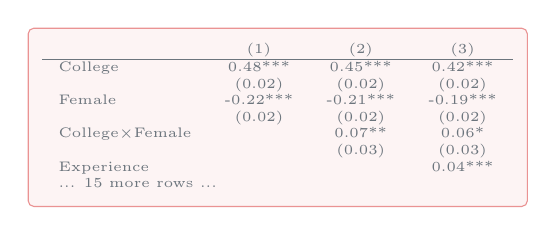
\begin{tikzpicture}
\node[draw=DeepRed!50, rounded corners=2pt, inner sep=5pt,
      text=WarmGray, font=\tiny, fill=DeepRed!5] {
    \begin{tabular}{lccc}
    & (1) & (2) & (3) \\
    \hline
    College & 0.48*** & 0.45*** & 0.42*** \\
    & (0.02) & (0.02) & (0.02) \\
    Female & -0.22*** & -0.21*** & -0.19*** \\
    & (0.02) & (0.02) & (0.02) \\
    College$\times$Female & & 0.07** & 0.06* \\
    & & (0.03) & (0.03) \\
    Experience & & & 0.04*** \\
    \multicolumn{4}{l}{\tiny ... 15 more rows ...}
    \end{tabular}
};
\end{tikzpicture}
\end{column}

\begin{column}{0.48\textwidth}
\textcolor{Teal}{\textbf{Good: Key Number Prominent}}\\[0.2cm]

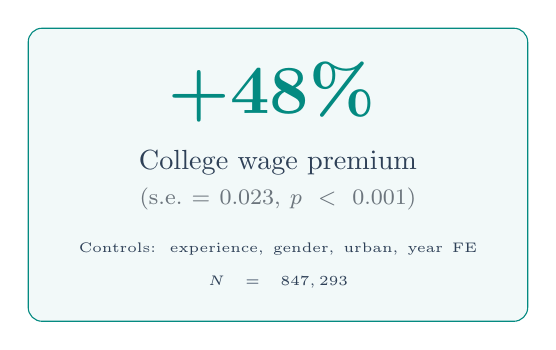
\begin{tikzpicture}
\node[draw=Teal, rounded corners=5pt, inner sep=12pt,
      text=DeepNavy, fill=Teal!5, text width=5.5cm, align=center] {
    {\fontsize{28}{32}\selectfont\bfseries\textcolor{Teal}{+48\%}}\\[0.3cm]
    \normalsize College wage premium\\[0.1cm]
    \footnotesize\graytext{(s.e.\ = 0.023, $p < 0.001$)}\\[0.4cm]
    \tiny Controls: experience, gender, urban, year FE\\
    $N = 847,293$
};
\end{tikzpicture}

\vspace{0.2cm}
\tealtext{\footnotesize The number that matters is unmistakable.}
\end{column}
\end{columns}
\end{frame}

\begin{frame}
\frametitle{Full Regression Table (When Needed)}
\framesubtitle{Returns to Education: Log Wage Regression}
\vspace{0.1cm}

\begin{center}
\renewcommand{\arraystretch}{1.2}
\footnotesize
\begin{tabular}{l >{\raggedleft\arraybackslash}p{2cm} >{\raggedleft\arraybackslash}p{1.6cm}}
\toprule
\rowcolor{DeepNavy!10}
\textbf{Variable} & \textbf{Coefficient} & \textbf{Std.\ Err.} \\
\midrule
College Degree & \textcolor{Teal}{\textbf{0.482***}} & (0.023) \\
Female & $-0.215$*** & (0.018) \\
\rowcolor{WarmOrange!10}
College $\times$ Female & \textcolor{WarmOrange}{\textbf{0.067**}} & (0.031) \\
Experience & 0.038*** & (0.003) \\
Experience$^2$/100 & $-0.065$*** & (0.008) \\
Urban & 0.124*** & (0.015) \\
Constant & 1.847*** & (0.042) \\
\midrule
\multicolumn{3}{l}{\scriptsize\graytext{$R^2 = 0.312$, $N = 847{,}293$, *** $p<0.01$, ** $p<0.05$}} \\
\bottomrule
\end{tabular}
\end{center}

\vspace{0.2cm}
\begin{center}
\footnotesize\tealtext{Key finding:} College premium is 48\%, but \emphcolor{larger for women} (+6.7pp).
\end{center}
\end{frame}

% -----------------------------------------------------------------------------
% FIGURE DESIGN PRINCIPLES
% -----------------------------------------------------------------------------
\begin{frame}
\frametitle{Figure Design: Labels and Self-Sufficiency}
\vspace{0.2cm}

Every figure should have:

\vspace{0.2cm}
\begin{columns}[T]
\begin{column}{0.48\textwidth}
\begin{itemize}
    \item \textbf{Title states the finding}\\
          \graytext{\scriptsize ``Policy X Increased Innovation'' not ``Figure 3''}
    \vspace{0.2cm}
    \item \textbf{Axis labels readable from back}\\
          \graytext{\scriptsize Larger than you think}
    \vspace{0.2cm}
    \item \textbf{Direct labeling}\\
          \graytext{\scriptsize Label lines, not legends}
\end{itemize}
\end{column}

\begin{column}{0.48\textwidth}
\begin{itemize}
    \item \textbf{Annotations on graphic}\\
          \graytext{\scriptsize ``Treatment begins here''}
    \vspace{0.2cm}
    \item \textbf{Source and notes}\\
          \graytext{\scriptsize Small text for later readers}
    \vspace{0.2cm}
    \item \textbf{Self-interpreting}\\
          \graytext{\scriptsize Grasp the point immediately}
\end{itemize}
\end{column}
\end{columns}

\vspace{0.3cm}
\begin{center}
\emphcolor{This is more work than defaults. It is work worth doing.}
\end{center}
\end{frame}

% -----------------------------------------------------------------------------
% BAD VS GOOD CHART
% -----------------------------------------------------------------------------
\begin{frame}
\frametitle{Visualization: Bad vs.\ Good}
\vspace{0.1cm}

\begin{columns}[T]
\begin{column}{0.48\textwidth}
\centering
\textcolor{DeepRed}{\textbf{Cluttered, Unfocused}}\\[0.2cm]
\includegraphics[width=\textwidth]{figures/fig6_bad_chart.pdf}

\vspace{0.2cm}
\graytext{\footnotesize Default colors, no focus, legend requires eye movement, what's the point?}
\end{column}

\begin{column}{0.48\textwidth}
\centering
\textcolor{Teal}{\textbf{Clear, Focused}}\\[0.2cm]
\includegraphics[width=\textwidth]{figures/fig6_good_chart.pdf}

\vspace{0.2cm}
\tealtext{\footnotesize One story, direct label, title states finding, eye knows where to go}
\end{column}
\end{columns}
\end{frame}

% -----------------------------------------------------------------------------
% TUFTE
% -----------------------------------------------------------------------------
\begin{frame}
\frametitle{Tufte's Critique---and Beyond}
\vspace{0.1cm}

\begin{columns}[T]
\begin{column}{0.48\textwidth}
\textcolor{DeepNavy}{\textbf{Tufte Is Right About}}\\[0.2cm]
\footnotesize
\begin{itemize}
    \setlength{\itemsep}{1pt}
    \item Bullet points fragment ideas
    \item Chartjunk obscures data
    \item Default templates encourage low-resolution thinking
    \item Bad decks proliferate
\end{itemize}
\end{column}

\begin{column}{0.48\textwidth}
\textcolor{WarmOrange}{\textbf{But His Critique Proves Too Much}}\\[0.2cm]
\footnotesize
\begin{itemize}
    \setlength{\itemsep}{1pt}
    \item If medium inherently corrupts, effective decks impossible
    \item \emphcolor{They're not.}
    \item Problem is misuse, not medium
    \item He evaluates as document, not performance
\end{itemize}
\end{column}
\end{columns}

\vspace{0.3cm}
\begin{center}
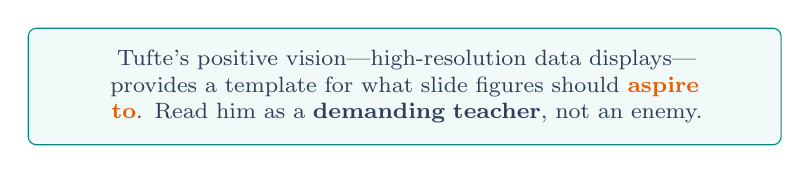
\begin{tikzpicture}
\node[draw=Teal, rounded corners=3pt, inner sep=8pt, text=DeepNavy, fill=Teal!5,
      text width=9cm, align=center, font=\footnotesize] {
    Tufte's positive vision---high-resolution data displays---provides
    a template for what slide figures should \emphcolor{aspire to}.
    Read him as a \textbf{demanding teacher}, not an enemy.
};
\end{tikzpicture}
\end{center}
\end{frame}

% -----------------------------------------------------------------------------
% CONCLUSION
% -----------------------------------------------------------------------------
\transitionslide{Conclusion}{Toward a Mature Theory}

\begin{frame}
\frametitle{What We've Established}
\vspace{0.1cm}

\begin{center}
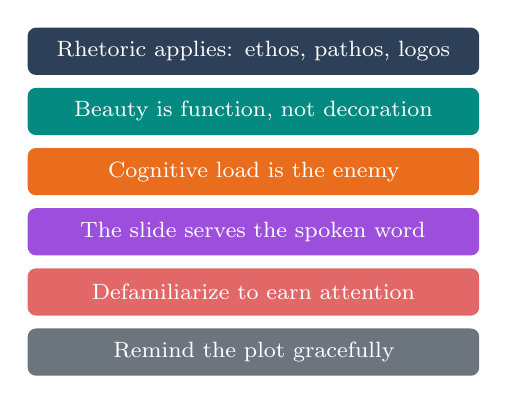
\begin{tikzpicture}[
    node distance=0.15cm,
    principle/.style={rectangle, rounded corners=3pt, minimum height=0.6cm,
                      text centered, font=\footnotesize, text=white, text width=5.5cm}
]
    \node[principle, fill=DeepNavy] (p1) {Rhetoric applies: ethos, pathos, logos};
    \node[principle, fill=Teal, below=0.15cm of p1] (p2) {Beauty is function, not decoration};
    \node[principle, fill=WarmOrange!90, below=0.15cm of p2] (p3) {Cognitive load is the enemy};
    \node[principle, fill=SoftPurple, below=0.15cm of p3] (p4) {The slide serves the spoken word};
    \node[principle, fill=DeepRed!70, below=0.15cm of p4] (p5) {Defamiliarize to earn attention};
    \node[principle, fill=WarmGray, below=0.15cm of p5] (p6) {Remind the plot gracefully};
\end{tikzpicture}
\end{center}

\vspace{0.3cm}
\begin{center}
\graytext{\footnotesize These principles persist. Their application varies with context.}
\end{center}
\end{frame}

\begin{frame}
\frametitle{The Contribution of LLMs}
\vspace{0.5cm}

\begin{center}

\begin{tikzpicture}
\node[text=DeepNavy, font=\large, text width=11cm, align=center] {
    What large language models contribute is perhaps not new principles\\
    but \emphcolor{newly available articulation}.
};
\end{tikzpicture}
\end{center}

\vspace{0.8cm}
\begin{columns}[T]
\begin{column}{0.3\textwidth}
\centering
\textcolor{Teal}{\textbf{Breadth}}\\[0.2cm]
\footnotesize More examples than any human encounters
\end{column}
\begin{column}{0.3\textwidth}
\centering
\textcolor{WarmOrange}{\textbf{Pattern Recognition}}\\[0.2cm]
\footnotesize Sensitivities to what works across contexts
\end{column}
\begin{column}{0.3\textwidth}
\centering
\textcolor{SoftPurple}{\textbf{Articulation}}\\[0.2cm]
\footnotesize Making explicit what practitioners know implicitly
\end{column}
\end{columns}

\vspace{0.8cm}
\begin{center}
\graytext{\small The tacit knowledge embedded in effective communication, now surface-able.}
\end{center}
\end{frame}

% -----------------------------------------------------------------------------
% FINAL SLIDE
% -----------------------------------------------------------------------------
{
\setbeamertemplate{footline}{}
\begin{frame}[plain]
\begin{tikzpicture}[remember picture,overlay]
    % Background
    \fill[DeepNavy] (current page.south west) rectangle (current page.north east);

    % Decorative elements
    \fill[Teal,opacity=0.2] ([xshift=4cm,yshift=-2cm]current page.north west) circle (6cm);
    \fill[WarmOrange,opacity=0.15] ([xshift=-3cm,yshift=3cm]current page.south east) circle (5cm);

    % Main message
    \node[anchor=center,text=white,font=\Large,text width=0.8\paperwidth,align=center]
        at ([yshift=1.5cm]current page.center) {
            Decks are how a large portion of human\\
            knowledge and decision-making now flows.
        };

    \node[anchor=center,text=LightGray,font=\large,text width=0.8\paperwidth,align=center]
        at ([yshift=-0.5cm]current page.center) {
            They deserve the serious analysis\\
            that earlier media have received.
        };

    % Final line
    \draw[WarmOrange,line width=2pt]
        ([yshift=-2cm,xshift=-4cm]current page.center) --
        ([yshift=-2cm,xshift=4cm]current page.center);

    \node[anchor=center,text=WarmOrange,font=\Large\bfseries]
        at ([yshift=-3cm]current page.center) {
            They deserve, at last, a rhetoric.
        };
\end{tikzpicture}
\end{frame}
}

\end{document}
